\chapter{经济效果评价指标}
\noindent{以货币单位计量的价值型指标:}\\
净现值、净年值、费用现值、费用年值等;\\
反映资金利用效率的效率型指标:\\
内部收益率、净现值指数、投资收益率等。

\section{(静态)投资回收期(Payback period)}
\subsection{概念}

从项目投建之日起,用项目各年的净收入(年收入减年支出)将全部投资收回所需的期限。

\begin{equation*}
\sum_{t=0}^{T_p}{(CI-CO)}_t = 0
\end{equation*}

(左边:累积净现金流量)
\begin{itemize}
    \item $T_p$ - 投资回收期
    \item $CI$ - 现金流入量
    \item $CO$ - 现金流出量
    \item $(CI-CO)_t$ - 第t年的净现金流量
\end{itemize}

\subsection{列表法}
如果投产或达产后各年的净收益不等,用列表法(累计净收益法)求得。

\subsection{投资回收期计算}

\begin{equation}
    T_p = (T - 1)+\frac{\sum_{t=0}^{T-1}{(CI-CO)}_t}{{(CI-CO)}_T}
\end{equation}

T为项目各年累积净现金流量首次为正值或零的年份。

案例:
\begin{figure}[h]
    \centering
    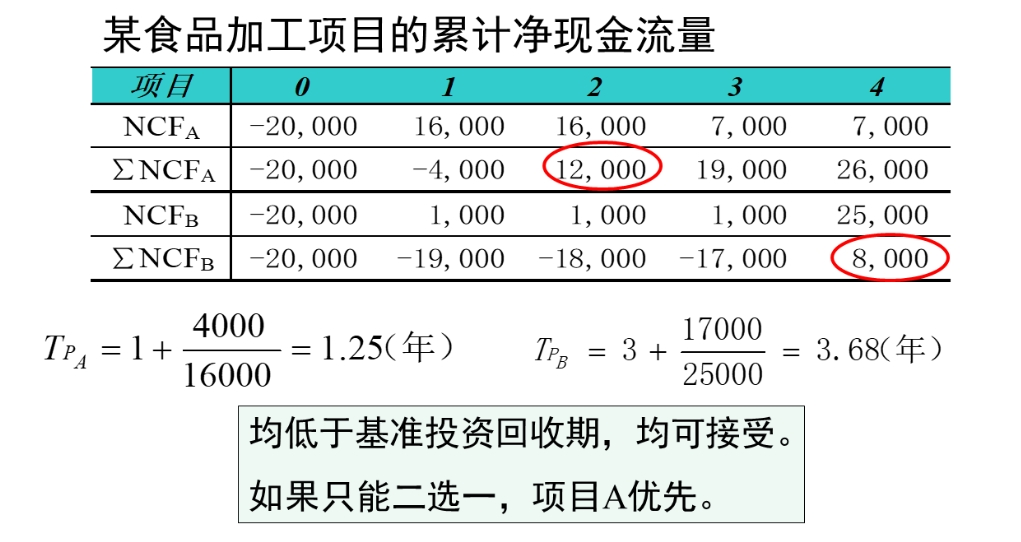
\includegraphics[width=\textwidth]{jxjll.png}
    \caption{例1:某食品加工项目的累计净现金流量}
    \label{fig:1}
\end{figure}

\subsection{指标评价}
\textbf{缺点}
\begin{itemize}
    \item 没有反映资金的时间价值;
    \item 未考虑回收期后的现金流,不能反映项目在整个投资期内的真实收益;
    \item 基准投资回收期的确定具有主观性。
\end{itemize}

\textbf{优点}
\begin{itemize}
    \item 简单、易懂;
    \item 在一定程度上反映了项目的经济性和风险大小。
\end{itemize}

\section{投资收益率(Return on investment)}

\subsection{总投资收益率(ROI)}

项目正常年份的息税前利润与投资总额的比值。
$$ROI=\mbox{息税前利润/总投资经济}$$

含义:项目投产后单位投资所创造的收益额。

\subsection{项目资本金净利润率(ROE)}

项目正常年份的年净利润与项目资本金的比值。
$$ROI=\frac{\mbox{净利润}}{\mbox{资本金经济}}$$

含义:项目投产后单位资本金所创造的收益额。

案例:
\begin{figure}[H]
    \centering
    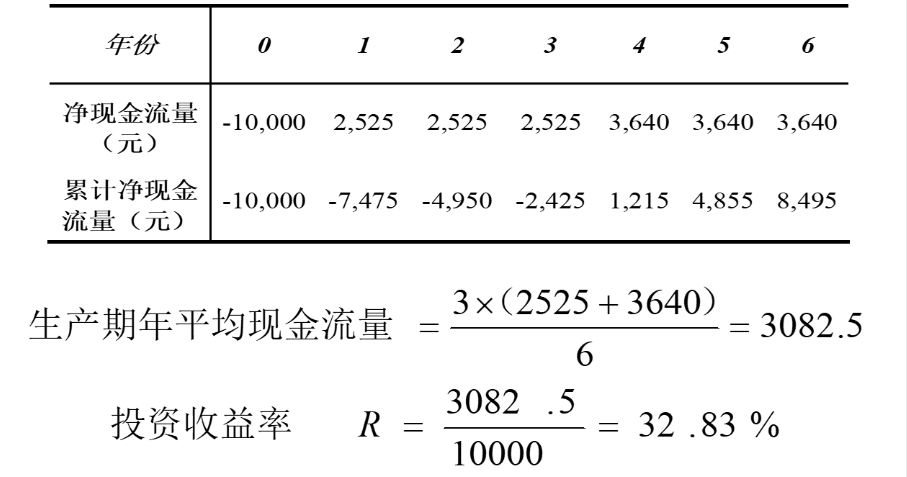
\includegraphics[width=\textwidth]{image/roi.png}
    \caption{例2:投资收益率}
    \label{fig:2}
\end{figure}

\subsection{判别准则}
设基准投资收益率为 $R$:
\begin{itemize}
    \item 若$R \geq R_b$,则项目可以考虑接受;
    \item 若$R \textless R_b$,则项目应予以拒绝。
\end{itemize}

\subsection{缺点}
\begin{itemize}
    \item 没有考虑时间价值;
    \item 当项目各年的经营状况不稳定时,该指标难以应用。
\end{itemize}

静态评价指标主要使用于\textbf{寿命周期较短且每期现金流量分布均匀}的技术方案评价,方案初选阶段。

\section{净现值(Net present value, NPV)}

\subsection{概念}
按一定的折现率将各年的净现金流量折现到期初的现值之和,反映项目净收益的现值。
\subsection{计算公式}
(不建议直接理解公式,建议跳过该部分,看例题)

$$NPV=\sum_{t=0}^{n}(CI-CO)_t(1+i_0)^{-t}=\sum_{t=0}^{n}NCF_t(1+i_0)^{-t}$$

\subsection{例题}
某工程项目总投资为5000万元,项目寿命期为10年,投资后1-10年内每年末可带来800万元的现金净流入,在10年末,还能回收资金200万元,基准折现率为12%,求项目的净现值,并判断该项目是否可行?\\
\textbf{答案:}$NPV = −5000 +800(P / A,12\%,10) + 200(P / F,12\%,10)= −415.60$(万元)

其中,$-5000$ 为现金流出现值,$800(P / A,12\%,10) + 200(P / F,12\%,10)$为现金流入现值。

那么,如何理解最后算得的结果呢?

算得的NPV值为$-415.60 \textless 0$,这表明如果投资该方案,则由该方案所带来的未来收益的现值小于现在投资的现值,即在一定折现率的条件下,未来收益不能全部回收现在的投资,项目在经济上不可行。

\subsection{判别标准}
若是一个方案,想要知道它可不可行,只需要把它的NPV值与0进行比较,若大于等于0则可行,小于0则不可行;而若是多个方案,只需要比较NPV值的大小,NPV值越大相对方案越优。

\subsection{确定项目的技术经济边界}
利用盈亏平衡原理的思路,可以根据决策需要建立技术经济边界分析模型(NPV=0),从技术角度反映经济问题。当项目盈亏平衡时,诸多影响项目技术经济效益的变量都存在一个临界值,即技术经济边界,合理确定这些边界将有利于项目的科学决策。

一个例子,上例中的变化基准折现率和净现值的计算,表格如下:
\begin{figure}[H]
    \centering
    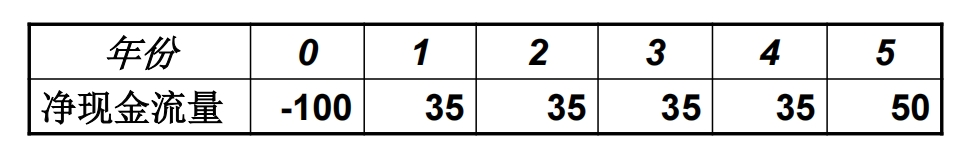
\includegraphics[width=0.9\textwidth]{image/年份-净现金流量.png}
    \label{fig:13}
\end{figure}
\begin{figure}[H]
    \centering
    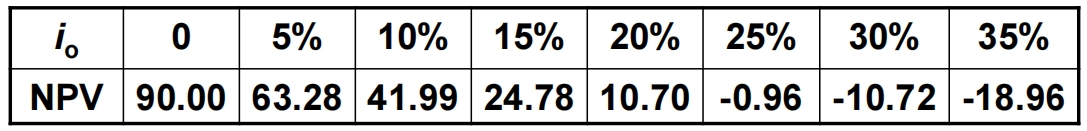
\includegraphics[width=0.9\textwidth]{image/i0-NPV.png}
    \label{fig:14}
\end{figure}

\begin{figure}[H]
    \centering
    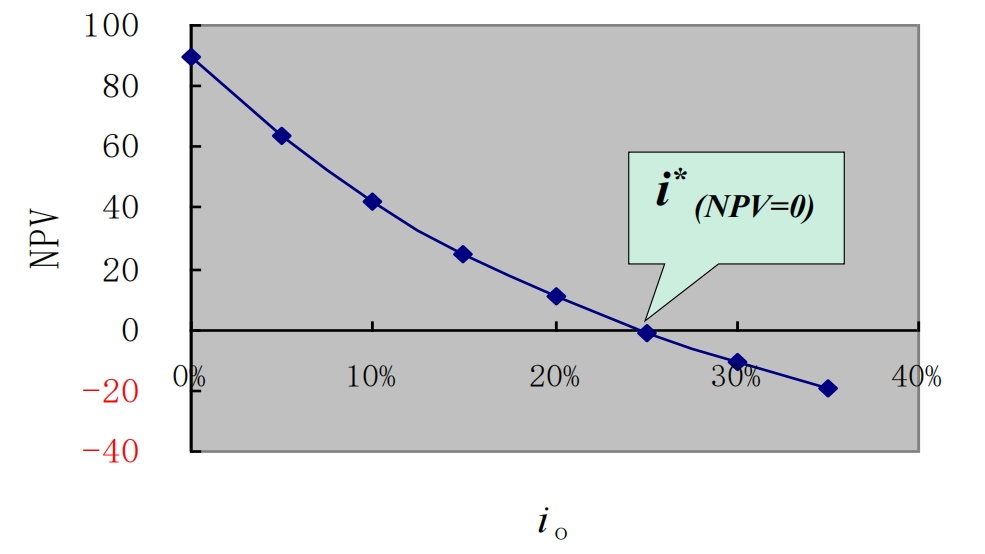
\includegraphics[width=\textwidth]{image/净现值与基准折现率的关系图示.png}
    \caption{净现值与基准折现率的关系图示}
    \label{fig:15}
\end{figure}

\textbf{净现值函数的特点:}同一净现金流量的净现值NPV随基准折现率$i_0$的增大而减小;基准折现率$i_0$定的越高,方案越可能被拒绝。

$i*$ 为折现率临界值,此时 NPV = 0;

i \textless i * 时, NPV \textless 0;

i \textgreater i * 时, NPV \textgreater 0。

\subsection{净现值对折现率的敏感性问题}
\subsubsection{举例}
下表列示了两个相互排斥的方案A、B的净现金流量,及其在折现率分别为10\%和20\%时的净现值。

\begin{table}[H]
\centering
\begin{tabular}{|c|c|c|c|c|c|c|c|c|}
\hline
    & 0   & 1   & 2   & 3   & 4   & 5   & NPV (10\%) & NPV (20\%) \\ \hline
A   & -230 & 100 & 100 & 100 & 50  & 50  & 83.91      & 24.81      \\ \hline
B   & -100 & 30  & 30  & 60  & 60  & 60  & 75.40      & 33.58      \\ \hline
\end{tabular}
\end{table}

当i=10\%时,$NPV_A \textgreater NPV_B$,则方案A优于方案B;

当i=20\%时,$NPV_A \textless NPV_B$,则方案B优于方案A。

此外,由表格后两列可以看出,方案A的净现值对折现率更敏感。

此现象,对投资决策的意义:

假设在一定的$i_0$和投资总限额$K_0$下,净现值大于0的项目有5个,其投资总额恰为$K_0$,故上述项目均被接受。按NPV的大小,其排序为A、B、C、D、E。

但若现在的投资总额必须压缩,减至$K_1$时,新选项目是否依然会遵循原排列顺序A、B、C...直至达到投资总额为止呢?一般说不会。

随着投资总额的压缩,应当提高基准折现率,但基准折现率由$i_0$提高到$i_1$后,由于各项目方案净现值对i的敏感性不同,原先净现值小的项目,其净现值现在可能大于原先净现值大的项目。

\section{净现值指数(Net present value index, NPVI)}
\subsection{概念}
项目的净现值与项目投资的现值之比。
\subsection{计算公式}
$$NPVI=\frac{NPV}{K_P}=\frac{NPV}{\sum_{t=0}^{n}K_t(1+i_0)^{-t}}$$

一个没见过的概念,$K_P$:项目投资现值。

NPV:考察的是资金利用的效果(绝对数),即总投资所能带来的净现值;

NPVI:可以考察资金利用的效率(相对比率),即单位投资所能带来的净现值。(排除了不同项目投资规模不同的影响)

\subsection{判别准则}
\noindent{\textbf{单一项目方案而言(与净现值相同)}:}

若NPVI \textgreater 0,则项目应予以接受;若NPVI \textless 0,则项目应予以拒绝。\\
\textbf{多方案比选时}:

净现值最大准则:NPV越大的方案相对越优。

注意:多方案比选时,NPV最大的方案,其NPVI不一定最大,此时,应根据NPV指标进行判断,选取NPV大的方案。简单理解:投资者追求的目标为在同等风险条件下获取的盈利最大。而净现值指标就是反映这种盈利的指标。\\
\textbf{例题:}项目各年净现金流量如下所示,基准折现率i=10\%,计算NPVI。
\begin{table}[H]
\centering
\begin{tabular}{|c|c|c|c|c|c|c|c|c|c|}
\hline
t   & 0 & 1 & 2 & 3 & 4  & 5  & 6  & 7   & 8      \\ \hline
NCF   & -100 & 50  & 45  & 45  & 45  & 45  & 45  & 45  & 45     \\ \hline
\end{tabular}
\end{table}
\textbf{答案:}$NPV =-100-50(P/F,10\%,1)+45(P/A,10\%,7)(P/F,10\%,1)=53.71$
$$NPVI=\frac{53.71}{100+50(P/F,10\%,1)}=0.37$$

\section{净年值(NAV)}

\subsection{概念}
通过资金等值换算,将项目净现值分摊到寿命期内各年的等额年值。
\subsection{公式}
$$NAV=NPV(A/P,I,N)$$
\subsection{判别标准}
对于单独一个项目:

$NAV \geq 0$:接受

NAV \textless 0:拒绝

就项目的评价结论而言,NPV,NAV是等效评价指标。\\
\textbf{例1:}某厂拟购置一台设备,购置费为100万元,预计使用五年后残值为20万元,在使用期5年内,由于使用这台机器每年可得收入50万元,而每年维修费等支出为22万元,若基准收益率为10\%,则净年值为?\\
\textbf{答案:}
\begin{figure}[H]
    \centering
    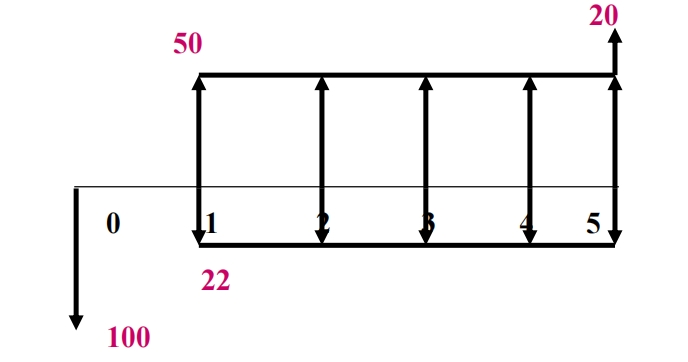
\includegraphics[width=0.7\textwidth]{image/NAV例题.png}
    \label{fig:16}
\end{figure}
\noindent{$NAV(10\%) = - 100(A/P,10\%,5)+28+20(A/F,10\%,5)= - 26.38 + 28 + 3.28= 4.9 \textgreater 0$}\\
$\because NAV(10\%) \textgreater 0$, \\
$\therefore$ 值得购置。\\
\textbf{例2:}(多选)关于净现值指数和净年值指标,说法正确的是(  )\\
A. 某方案,若净现值大于0,则净现值指数也大于0\\
B. 净现值指数是指单位投资现值所能带来的净现值\\
C. 多方案比较时,净现值指数可以作为净现值的辅助评价指标\\
D. 净年值体现项目生产期内每年的等额的超额收益\\
\textbf{答案:}ABC

\section{费用现值(PC)与费用年值(AC)}
\subsection{适用范围}
在对\textbf{多个方案}比较选优时,如果诸方案\textbf{产出价值相同},或者诸方案能够满足同样需要,其产出效益\textbf{难以用价值形态(货币)衡量}时,可以通过对各方案费用现值或费用年值比较进行选择。

\subsection{计算公式}
\subsubsection{费用现值的表达式:}
$$PC=\sum_{t=0}^{n}CO_{t}(P/F,i_0,t)$$

\subsubsection{费用年值表达式:}
$$AC=PC(A/P,i_0,n)=\sum_{t=0}^{n}CO_{t}(P/F,i_0,t)(A/P,i_0,n)$$

\subsection{判断准则}
费用现值和费用年值指标只能用于多个方案的比选,\textbf{费用现值或费用年值最小}的方案为优。

费用现值和费用年值的关系,与前述净现值和净年值的关系一样,故就评价结论而言,二者是等效评价指标。

\textbf{注意:PC与AC不能评价项目是否可行,只能用于多方案选优。}\\
\textbf{例1:}有两台功能相同、但费用不同的设备,试分析应选购哪台设备?(单位:万元,$i_0 = 15\%$)

\begin{table}[H]
\centering
\begin{tabular}{|c|c|c|c|c|}
\hline
设备 & 购置费用 & \multicolumn{2}{c|}{年运行费} & 第6年末残值 \\ \hline
    &           & 前3年每年 & 后3年每年 &              \\ \hline
A   & 10        & 5         & 6         & 4            \\ \hline
B   & 7.5       & 6         & 6         & 0            \\ \hline
\end{tabular}
\caption{设备购置及年运行费用和残值表}
\end{table}

\noindent{\textbf{答案:}}\\
$AC_A(15\%) = 10(A/P,15\%,6) + 5 + [1(F/A,15\%,3) – 4](A/F,15\%,6)= 7.58$(万元)\\
$AC_B(15\%) = 7.5 (A/P,15\%,6) + 6 = 7.98$(万元)\\
$\because AC_A(15\%) < AC_B(15\%)$,\\
$\therefore$ 应选择A设备;\\
$PC_A(15\%)=7.58 (P/A,15\%,6) =7.58×3.784=28.68$(万元)\\
$PC_B(15\%)=7.98 (P/A,15\%,6) =7.98×3.784=30.20$(万元)\\
$\because PC_A(15\%) < PC_B(15\%)$\\
$\therefore$ 应选择A设备。\\
\textbf{例2:}关于PC、AC指标,说法错误的是( )\\
A. PC、AC的指标值一般都小于0\\
B. PC、AC可用于单一方案的评判\\
C. 利用PC、AC指标时,可不考虑残值收入\\
D. PC、AC评判寿命期相等的方案时,是等效的\\
\textbf{答案:}ABC

\section{内部收益率(Internal rate of return, IRR)}
\subsection{概念}
净现值为零时的折现率(IRR)。
\begin{figure}[H]
    \centering
    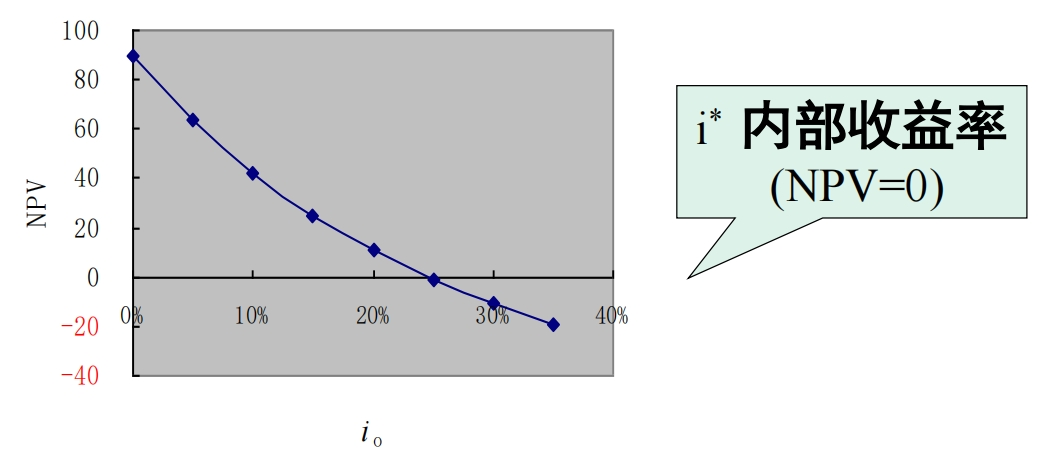
\includegraphics[width=\textwidth]{image/内部收益率IRR.png}
    \label{fig:17}
\end{figure}

\subsection{计算公式}
此处略,因为一元高次方程解起来太复杂,所以直接看例题,学会使用“试算内插法”即可。

\subsection{内部收益率计算的试插法}
\begin{figure}[H]
    \centering
    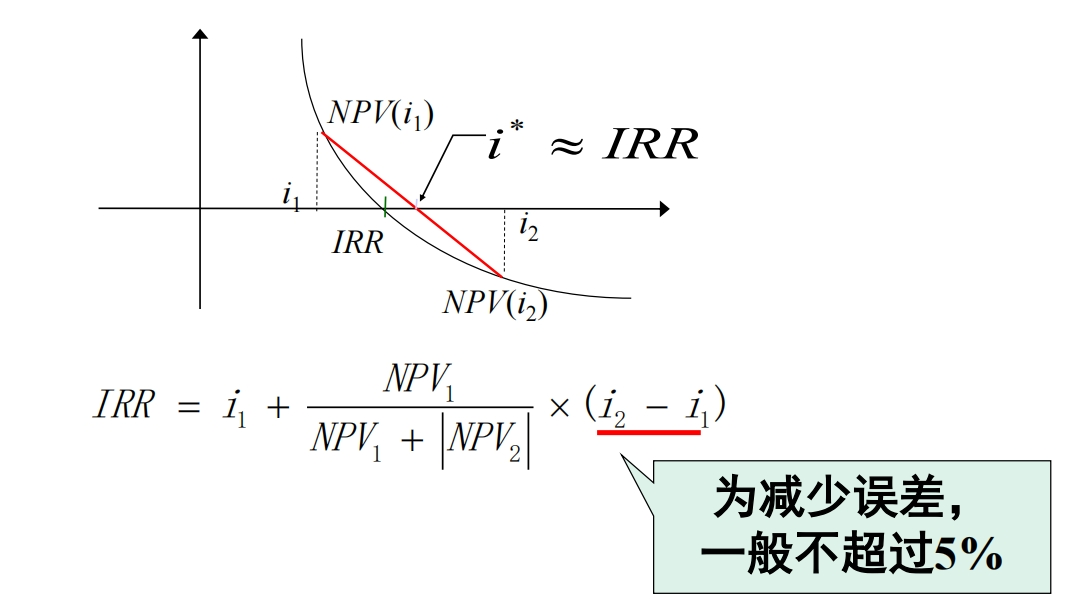
\includegraphics[width=0.9\textwidth]{image/试算内插法.png}
    \label{fig:18}
\end{figure}

\noindent{\textbf{例1:}}
\begin{table}[H]
\centering
\begin{tabular}{|c|c|c|c|c|c|c|}
\hline
t   & 0 & 1 & 2 & 3 & 4  & 5  \\ \hline
NCF   & -20000 & 6000  & 6000  & 7000  & 7000  & 10000   \\ \hline
\end{tabular}
\end{table}
\noindent{\textbf{答案:}}\\
$NPV = −20000 + 6000(P/ A,i,2) + 7000(P/ A,i,2)(P/ F,i,2) +10000(P/ F,i,5) = 0$\\
$i_1=20\%, NPV_1=612$\\ 
$i_2=25\%, NPV_2=-1632$
$$IRR=20\%+\frac{612-0}{612-(-1632)} \times 5\%=21.36\%$$
21.26\%就是项目自身的收益率。\\
\textbf{例2:}
\begin{table}[H]
\centering
\begin{tabular}{|c|c|c|c|c|c|c|}
\hline
t   & 0 & 1 & 2 & 3 & 4  & 5  \\ \hline
NCF   & -20000 & 7800  & 7800  & 7800  & 7800  & 7800   \\ \hline
\end{tabular}
\end{table}
\noindent{\textbf{答案:}}\\
$NPV = −20000 + 7800(P/ A,IRR,5) = 0$\\
$(P/A,IRR,5) = 2.5641$\\
\textbf{试插:}\\
$(P/A,25\%,5)=2.6893$\\
$(P/A,30\%,5)=2.4356$
$$IRR=25\%+\frac{2.6893-2.5641}{2.6893-2.4356} \times 5\% =27.47\%$$

\subsection{判别准则($i_0$为基准折现率/收益率/贴现率)}
$IRR \geq i_0$,项目可以接受;
$IRR \textless i_0$ ,项目应该拒绝。

基准收益率是投资者要求的最低投资收益率,如果项目的收益率大于或等于基准收益率,则项目经济可行;如果项目的收益率低于基准收益率,则项目不经济。

对某一方案而言:$IRR \geq i_0$, 即$NPV \geq 0$ ;$IRR \textless i_0$,即$NPV \textless 0$

\subsection{内部收益率隐含的经济意义}
\noindent{\textbf{表述一:}}

在项目的整个寿命期内,按利率i*=IRR来计算,会始终存在未能收回的投资,只有在寿命期结束时,投资恰好被全部收回。即在项目寿命期内,项目始终处于“偿付”未被收回的投资的状况。\\
\textbf{表述二:}

IRR是项目寿命期内没有回收投资的盈利率。\\
\textbf{例1:}
\begin{table}[H]
\centering
\begin{tabular}{|c|c|c|c|c|c|c|}
\hline
t   & 0 & 1 & 2 & 3 & 4  & 5  \\ \hline
NCF   & -20000 & 7800  & 7800  & 7800  & 7800  & 7800   \\ \hline
\end{tabular}
\end{table}
其IRR=27.47\%。当以IRR为折现率时,一直到项目寿命期末,才将未收回的投资全部回收。当以IRR为折现率时,可求得该投资项目在寿命期内,对应于每一年的净现值。\\
\textbf{例2:}某公司购买一台设备投资100000万元,寿命期为4年,每年年末的净收益分别是40000,37000,24000,22000元,可求得内部收益率等于10\%。它表示在寿命期内未被收回的投资在10\%的利率下,项目寿命期终了时能被完全收回。

内部收益率指标是一个相对指标,未考虑投资规模等对投资决策的影响,因此有时会做出错误的选择。如:投资期内项目净现金流入多次改变符号时、投资项目初始投资额不等时、投资项目现金流量发生的时间不同时。

\section{动态投资回收期}
\subsection{概念}
指项目累积净现金流量现值为零所需要的时间。(克服静态投资回收期未考虑资金时间价值的缺点)

\subsection{计算公式}
$$\sum_{t=0}^{T_P}(CI-CO)_t(1+i_0)^{-t}=0$$

\subsection{判别准则}
设Tb*为基准动态投资回收期,
若TP* $\leq$ Tb*,则项目可以考虑接受;
若TP* $\textgreater$ Tb*,则项目应予以拒绝。

